\documentclass{article}
% \documentclass[12pt, draftcls, journal]{IEEEtran}
\usepackage{amsmath}
\usepackage{amsfonts}
\usepackage{hyperref}
\usepackage{graphicx}
\usepackage{setspace}
\usepackage{fancyhdr}
\usepackage{float}
\usepackage[a4paper, margin=1in]{geometry}


\newcommand{\R}{\mathbb{R}}

\pagestyle{fancy}
\begin{document}



\author{kipngeno koech - bkoech}
\title{Homework 4 - Math Foundation for Machine Learning Engineers}   
\maketitle

\medskip


\section{Warm Up Derivatives (10 Points)}
Compute the first and second derivatives of the following functions:
\begin{enumerate}
    \item $f(x) = \mathbf{M}^\top \mathbf{M} \mathbf{x}$, where $\mathbf{x} \in \mathbb{R}^m$ and $\mathbf{M} \in \mathbb{R}^{m \times m}$. What happens if $\mathbf{M} = \mathbf{M}^\top$?
    \\ first derivative:
    \[
    \frac{\partial f}{\partial x} = \mathbf{M}^\top \mathbf{M}
    \]
    second derivative:
    \[
    \frac{\partial^2 f}{\partial x^2} = 0
    \]
    if $M = M^\top$: then 
    \item $f(\mathbf{X}) = \text{tr}(\mathbf{M}\mathbf{X})$, where $\mathbf{M} \in \mathbb{R}^{m \times n}$ and $\mathbf{X} \in \mathbb{R}^{n \times m}$, and $\text{tr}$ is the trace of a square matrix.
    \item $f(\mathbf{X}) = \text{tr}(\mathbf{X} \mathbf{X}^\top)$, where $\mathbf{X} \in \mathbb{R}^{n \times n}$, and $\text{tr}$ is the trace of a square matrix.
    \item $f(\mathbf{X}) = \mathbf{a}^\top \mathbf{X} \mathbf{b}$, where $\mathbf{X} \in \mathbb{R}^{m \times n}$, $\mathbf{a} \in \mathbb{R}^m$ and $\mathbf{b} \in \mathbb{R}^n$.
    \item $f(\mathbf{X}) = \mathbf{a}^\top \mathbf{X}^\top \mathbf{X} \mathbf{b}$, where $\mathbf{X} \in \mathbb{R}^{n \times m}$, $\mathbf{a} \in \mathbb{R}^m$ and $\mathbf{b} \in \mathbb{R}^m$.
\end{enumerate}

\section{Ridge Regression (20 Points)}
In ordinary least squares (OLS) regression, we seek to minimize the sum of squared residuals:

\begin{align}
\min_{\boldsymbol{\beta}} \|\mathbf{y} - \mathbf{X} \boldsymbol{\beta} \|^2
\end{align}

where $\mathbf{y}$ is the vector of observed target values and $\mathbf{X}$ is the matrix of input features.

We have shown in class and during recitation that the optimal parameters for OLS regression can be given by:

\begin{align}
\boldsymbol{\beta} = (\mathbf{X}^\top \mathbf{X})^{-1} \mathbf{X}^\top \mathbf{y}
\end{align}

However, OLS can have several issues:
\begin{itemize}
    \item The matrix $\mathbf{X}^\top \mathbf{X}$ may be non-invertible or ill-conditioned when features are correlated (multicollinearity).
    \item OLS can lead to overfitting, especially when the number of features is large relative to the number of observations.
    \item OLS is sensitive to outliers since the cost function is based on squared residuals.
\end{itemize}

\subsection{Ridge Regression Solution (10 Points)}
Ridge regression modifies the OLS objective function by adding a penalty term:

\begin{align}
\min_{\boldsymbol{\beta}} \left( \|\mathbf{y} - \mathbf{X} \boldsymbol{\beta}\|^2 + \lambda \|\boldsymbol{\beta}\|^2 \right)
\end{align}

where $\lambda$ is a regularization parameter that controls the strength of the penalty. Show that the optimal parameters $\boldsymbol{\beta}$ is:

\begin{align}
\boldsymbol{\beta} = (\mathbf{X}^\top \mathbf{X} + \lambda \mathbf{I})^{-1} \mathbf{X}^\top \mathbf{y}
\end{align}

where $\mathbf{I}$ is the identity matrix. This ensures that the solution is always unique (since $\mathbf{X}^\top \mathbf{X} + \lambda \mathbf{I}$ is always invertible) and less sensitive to collinear features or outliers.

\[
\min_{\boldsymbol{\beta}} \left( \|\mathbf{y} - \mathbf{X} \boldsymbol{\beta}\|^2 + \lambda \|\boldsymbol{\beta}\|^2 \right)
\]
\[
\min_{\boldsymbol{\beta}} \left( (\mathbf{y} - \mathbf{X} \boldsymbol{\beta})^\top (\mathbf{y} - \mathbf{X} \boldsymbol{\beta}) + \lambda \boldsymbol{\beta}^\top \boldsymbol{\beta} \right)
\]
\[
\min_{\boldsymbol{\beta}} \left( \mathbf{y}^\top \mathbf{y} - \mathbf{y}^\top \mathbf{X} \boldsymbol{\beta} - \boldsymbol{\beta}^\top \mathbf{X}^\top \mathbf{y} + \boldsymbol{\beta}^\top \mathbf{X}^\top \mathbf{X} \boldsymbol{\beta} + \lambda \boldsymbol{\beta}^\top \boldsymbol{\beta} \right)
\]
\[
\min_{\boldsymbol{\beta}} \left( \mathbf{y}^\top \mathbf{y} - 2 \mathbf{y}^\top \mathbf{X} \boldsymbol{\beta} + \boldsymbol{\beta}^\top \mathbf{X}^\top \mathbf{X} \boldsymbol{\beta} + \lambda \boldsymbol{\beta}^\top \boldsymbol{\beta} \right)
\]
\[
\frac{\partial}{\partial \boldsymbol{\beta}} \left( \mathbf{y}^\top \mathbf{y} - 2 \mathbf{y}^\top \mathbf{X} \boldsymbol{\beta} + \boldsymbol{\beta}^\top \mathbf{X}^\top \mathbf{X} \boldsymbol{\beta} + \lambda \boldsymbol{\beta}^\top \boldsymbol{\beta} \right) = 0
\]
\[
-2 \mathbf{X}^\top \mathbf{y} + 2 \mathbf{X}^\top \mathbf{X} \boldsymbol{\beta} + 2 \lambda \boldsymbol{\beta} = 0
\]
\[
\mathbf{X}^\top \mathbf{X} \boldsymbol{\beta} + \lambda \boldsymbol{\beta} = \mathbf{X}^\top \mathbf{y}
\]
\[
(\mathbf{X}^\top \mathbf{X} + \lambda \mathbf{I}) \boldsymbol{\beta} = \mathbf{X}^\top \mathbf{y}
\]
\[
\boldsymbol{\beta} = (\mathbf{X}^\top \mathbf{X} + \lambda \mathbf{I})^{-1} \mathbf{X}^\top \mathbf{y}
\]

\subsection{Coding Ridge Regression (10 Points)}
Complete the Ridge Regression code in the attached notebook and report the effect of changing the bias parameter.

\section{Artificial Neural Network (60 Points)}
In our recent recitation, we discussed artificial neural networks (ANNs) as complex functions that represent the intricate architecture of the human brain’s neural network. These functions are subject to optimization to improve performance, a task often achieved through backpropagation and gradient descent, wherein the network adjusts its weights to minimize error and enhance accuracy in tasks such as classification and prediction.

We can summarize optimizing the model parameters (weights and biases) as follows:

Learning in deep neural networks using Gradient Descent can be summarized as follows:
\begin{enumerate}
    \item \textbf{Initialization:} Initialize the network’s weights and biases, often randomly or by some heuristic.
    \item \textbf{Forward Pass:} Input data is passed through the network. Each neuron computes a weighted sum of the inputs and a bias, followed by an activation function.
    \item \textbf{Loss Calculation:} The network’s prediction is compared to the true outcome using a loss function to calculate the error.
    \item \textbf{Backward Pass (Backpropagation):} Calculate the gradient of the loss function with respect to each parameter using the chain rule.
    \item \textbf{Gradient Descent:} Adjust the parameters in the opposite direction of the gradient to minimize the error.
    \item \textbf{Update Parameters:} Update the weights by the equation:
    \[
    w_{\text{new}} = w_{\text{old}} - \alpha \cdot \nabla_w L,
    \]
    where $\alpha$ is the learning rate, $\nabla_w L$ is the gradient of the loss with respect to the weights, and $w$ represents the weights.
    \item \textbf{Iteration:} Repeat the forward pass, loss calculation, backpropagation, and parameter update until the loss converges or a stopping criterion is met.
\end{enumerate}

\subsection{Chain Rule and Backpropagation (20 Points)}
Consider a network structured with two input nodes, two hidden nodes, and a single output node. Nodes 3 and 4 use the sigmoid and tanh functions, respectively. The remaining nodes are designed with linear activation, meaning that their outputs are directly proportional to
their inputs.

\begin{center}
    
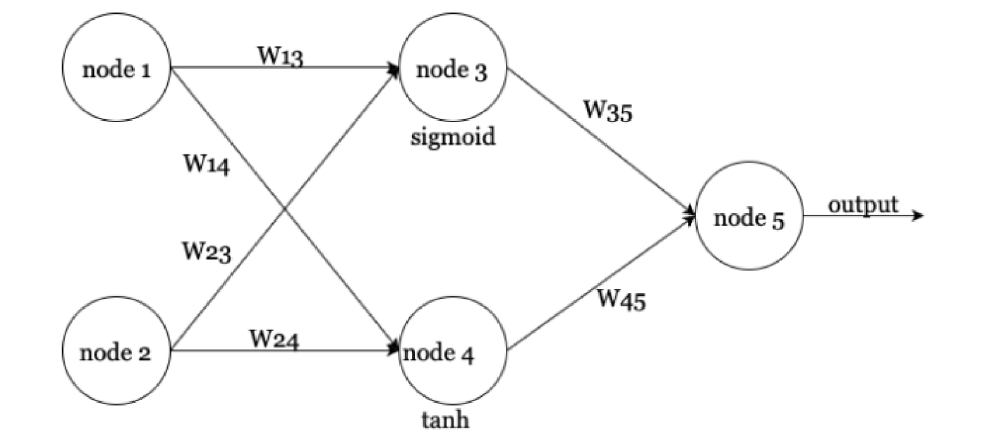
\includegraphics[scale=0.4]{nn.png}
\end{center}

We will follow the procedures described in the previous section.

\begin{enumerate}
\item \textbf{Initialization: } 
The weights are assigned as follows:


The inputs of node 1 and node 2 are 1.0 and -1.0 respectively.
\[
W_{13} = 1, \quad W_{14} = -1, \quad W_{23} = 2, \quad W_{24} = -3, \quad W_{35} = 2, \quad W_{45} = -1.
\]

The hyperbolic tangent function is given by:
\[
\tanh(x) = \frac{e^{2x} - 1}{e^{2x} + 1}
\]

The sigmoid function is:
\[
\sigma(x) = \frac{1}{1 + e^{-x}}
\]

There is no bias term in this network.


    \item \textbf{Forward Pass (5 Points):} Compute the output of node 5.
    \[
    \text{Node 3: } a_3 = \sigma(W_{13} \cdot x_1 + W_{23} \cdot x_2) \quad \text{Node 4: } a_4 = \tanh(W_{14} \cdot x_1 + W_{24} \cdot x_2) \quad \text{Node 5: } a_5 = W_{35} \cdot a_3 + W_{45} \cdot a_4
    \]
    \[
    \text{Node 3: } a_3 = \sigma(1 \cdot 1 + 2 \cdot -1) \quad \text{Node 4: } a_4 = \tanh(-1 \cdot 1 - 3 \cdot -1) \quad \text{Node 5: } a_5 = 2 \cdot a_3 + -1 \cdot a_4
    \]
    \[
    \text{Node 3: } a_3 = \sigma(1 - 2) \quad \text{Node 4: } a_4 = \tanh(-1 + 3) \quad \text{Node 5: } a_5 = 2 \cdot a_3 + -1 \cdot a_4
    \]
    \[
    \text{Node 3: } a_3 = \sigma(-1) \quad \text{Node 4: } a_4 = \tanh(2) \quad \text{Node 5: } a_5 = 2 \cdot a_3 + -1 \cdot a_4
    \]
    \[
    \text{Node 3: } a_3 = \frac{1}{1 + e^{-x}} \quad \text{Node 4: } a_4 = \frac{e^{2x} - 1}{e^{2x} + 1} \quad \text{Node 5: } a_5 = 2 \cdot a_3 + -1 \cdot a_4
    \]
    \[
    \text{Node 3: } a_3 = \frac{1}{1 + e^{1}} \quad \text{Node 4: } a_4 = \frac{e^{4} - 1}{e^{4} + 1} \quad \text{Node 5: } a_5 = 2 \cdot a_3 + -1 \cdot a_4
    \]
    \[
    \text{Node 3: } a_3 = \frac{1}{1 + 2.71828} \quad \text{Node 4: } a_4 = \frac{54.59815 - 1}{54.59815 + 1} \quad \text{Node 5: } a_5 = 2 \cdot a_3 + -1 \cdot a_4
    \]
    \[
    \text{Node 3: } a_3 = 0.26894 \quad \text{Node 4: } a_4 = 0.96403 \quad \text{Node 5: } a_5 = 2 \cdot 0.26894 + -1 \cdot 0.96403
    \]
    \[
    \text{Node 3: } a_3 = 0.26894 \quad \text{Node 4: } a_4 = 0.96403 \quad \text{Node 5: } a_5 = 0.53788 - 0.96403
    \]
    \[
     \text{Node 5: } a_5 = \textbf{-0.42614473734}
    \]
    \item \textbf{Loss Calculation (2 Points):} The loss function is $L(y, \hat{y}) = (\hat{y} - y)^2$, where $y$ is the output of node 5 (answer from previous part) and $\hat{y}$ is the desired output. In this part, we let $\hat{y} = 1.0$. Compute the loss of the network.
    \[
    L = (\hat{y} - y)^2 = (1.0 - (-0.42615))^2 = (1.42615)^2 = \textbf{2.03388881183}
    \]
    \item \textbf{Backpropagation (8 Points):} Calculate the gradient of the loss function with respect to each parameter
using the chain rule. Remember the parameters are normally the weights and biases, but here we
don’t use a bias so the parameters are the weights. So for each weight, write down the derivative with
respect to that weight
    \[ 
        \frac{\partial L}{\partial W_{35}}, \quad \frac{\partial L}{\partial W_{45}}, \quad \frac{\partial L}{\partial W_{13}}, \quad \frac{\partial L}{\partial W_{14}}, \quad \frac{\partial L}{\partial W_{23}}, \quad \frac{\partial L}{\partial W_{24}} 
    \]
    derivative w.r.t to node 5:
    \[
    \frac{\partial L}{\partial a_5} = -2 \cdot (\hat{y} - y) = -2 \cdot (1.0 - (-0.42615)) = \textbf{-2.8522894747}
    \]
    derivative w.r.t to $W_{35}$:
    \[
    \frac{\partial L}{\partial W_{35}} = \frac{\partial L}{\partial a_5} \cdot \frac{\partial a_5}{\partial W_{35}} = -2.8522894747 \cdot a_3 = -2.852 \cdot 0.26894142137 = \textbf{-0.76709878548}
    \]
    derivative w.r.t to $W_{45}$:
    \[
    \frac{\partial L}{\partial W_{45}} = \frac{\partial L}{\partial a_5} \cdot \frac{\partial a_5}{\partial W_{45}} = -2.8522894747 \cdot a_4 = -2.8522894747 \cdot 0.96402758008 = \textbf{-2.74968571998}
    \]
    derivative w.r.t to node 4:
    \[
    \frac{\partial L}{\partial a_4} = \frac{\partial L}{\partial a_5} \cdot \frac{\partial a_5}{\partial a_4} = -2.8522894747 \cdot W_{45} = -2.8522894747 \cdot -1 = \textbf{2.8522894747}
    \]
    derivative w.r.t to tanh:
    \[
    \frac{\partial L}{\partial tanh} = \frac{\partial L}{\partial a_4} \cdot \frac{\partial a_4}{\partial tanh} = 2.8522894747 \cdot \tanh'(W_{14} \cdot x_1 + W_{24} \cdot x_2) 
    \]
    \[
    = 2.8522894747 * (1- 0.96402758008^2) = 2.8522894747 * (0.07065082485 ) = \textbf{0.20151660408}
    \]
    derivative w.r.t to $W_{14}$:
    \[
    \frac{\partial L}{\partial W_{14}} = \frac{\partial L}{\partial tanh} \cdot \frac{\partial a_4}{\partial W_{14}} = 0.20151660408 \cdot x_1 = 0.20151660408 \cdot 1 = \textbf{0.20151660408}
    \]
    derivative w.r.t to $W_{24}$:
    \[
    \frac{\partial L}{\partial W_{24}} = \frac{\partial L}{\partial tanh} \cdot \frac{\partial a_4}{\partial W_{24}} = 0.20151660408 \cdot x_2 = 0.20151660408 \cdot -1 = \textbf{-0.20151660408}
    \]
    derivative w.r.t to node 3:
    \[
    \frac{\partial L}{\partial a_3} = \frac{\partial L}{\partial a_5} \cdot \frac{\partial a_5}{\partial a_3} = -2.8522894747 \cdot W_{35} = -2.8522894747 \cdot 2 = \textbf{-5.7045789494}
    \]
    N/B: the derivative of the sigmoid function is $\sigma'(x) = \sigma(x)(1 - \sigma(x))$
    \\ derivative w.r.t to sigmoid:
    \[
    \frac{\partial L}{\partial \sigma} = \frac{\partial L}{\partial a_3} \cdot \frac{\partial a_3}{\partial \sigma} = -5.7045789494 \cdot \sigma'(W_{13} \cdot x_1 + W_{23} \cdot x_2)
    \]
    \[
    = -5.7045789494 \cdot 0.26894142137 \cdot (1 - 0.26894142137) = -5.7045789494 \cdot 0.26894142137 \cdot 0.73105857863
    \]
    \[
        = \textbf{-1.12158829557}
    \]
    derivative w.r.t to $W_{13}$:
    \[
    \frac{\partial L}{\partial W_{13}} = \frac{\partial L}{\partial \sigma} \cdot \frac{\partial a_3}{\partial W_{13}} = -1.12158829557 \cdot x_1 = -1.12158829557 \cdot 1 = \textbf{-1.12158829557}
    \]
    derivative w.r.t to $W_{23}$:
    \[
    \frac{\partial L}{\partial W_{23}} = \frac{\partial L}{\partial \sigma} \cdot \frac{\partial a_3}{\partial W_{23}} = -1.12158829557 \cdot x_2 = -1.12158829557 \cdot -1 = \textbf{1.12158829557}
    \]
\item \textbf{Gradient Descent and Parameter Update (5 Points):}Use the gradient descent optimization
technique to update the parameters. Since we are minimizing the loss, we will go in the opposite
direction of the gradient.
    \[
    w_{\text{new}} = w_{\text{old}} - \alpha \cdot \nabla_w L,
    \]
    
    use learning rate $\alpha = 0.1$. 
    
    After one iteration, report the weight values in the table below (keep only 2 decimal digits): example
in table below
\\ updating weights:
\\ updating $W_{13}$:
    \[
    W_{13_{\text{new}}} = W_{13_{\text{old}}} - \alpha \cdot \frac{\partial L}{\partial W_{13}} = 1 - 0.1 \cdot -1.12158829557 = \textbf{1.11215882956}
    \]
updating $W_{14}$:
    \[
    W_{14_{\text{new}}} = W_{14_{\text{old}}} - \alpha \cdot \frac{\partial L}{\partial W_{14}} = -1 - 0.1 \cdot 0.20151660408 = \textbf{0.97984833959}
    \]
updating $W_{23}$:
    \[
    W_{23_{\text{new}}} = W_{23_{\text{old}}} - \alpha \cdot \frac{\partial L}{\partial W_{23}} = 2 - 0.1 \cdot 1.12158829557 = \textbf{1.88784117044}
    \]
updating $W_{24}$:
    \[
    W_{24_{\text{new}}} = W_{24_{\text{old}}} - \alpha \cdot \frac{\partial L}{\partial W_{24}} = -3 - 0.1 \cdot -0.20151660408 = \textbf{-2.97984833959}
    \]
updating $W_{35}$:
    \[
    W_{35_{\text{new}}} = W_{35_{\text{old}}} - \alpha \cdot \frac{\partial L}{\partial W_{35}} = 2 - 0.1 \cdot -0.76709878548 = \textbf{2.07670987855}
    \]
updating $W_{45}$:
    \[
    W_{45_{\text{new}}} = W_{45_{\text{old}}} - \alpha \cdot \frac{\partial L}{\partial W_{45}} = -1 - 0.1 \cdot -2.74968571998 = \textbf{-0.72503142800}
    \]
    \begin{center}
        \begin{tabular}{|c|c|c|c|c|c|}
        \hline
        $W_{13}$ & $W_{14}$ & $W_{23}$ & $W_{24}$ & $W_{35}$ & $W_{45}$ \\ \hline
        1.11   & 0.98    & 1.88    & -2.98    & 2.08   &  0.73  \\ \hline
        \end{tabular}
    \end{center}
\end{enumerate}

\subsection{Checkpoint 1}
\begin{enumerate}
    \item  Are you comfortable calculating the derivatives ? $\textbf{Yes}$
\item Are you comfortable applying the gradient descent ? $\textbf{Yes}$
\item Are you comfortable completing the previous section ? $\textbf{Yes}$
\end{enumerate}

If your answer is NO, please post on piazza, attend office hour for a TA to help you understand.
Do not move to next section. You might see this in your exam.


If your answer is Yes, congratulations, you learned some of the basics of neural network and it will help you
in the Introduction to deep learning and Introduction to machine learning course.

\subsection{Bonus (5 Points)}
Run another iteration (5 points) Use the updated weights of previous section. However the inputs of
node 1 and node 2 are 2.0 and -2.0 respectively, the desired output is 2. What is your predicted output, and
what is your updated weights ?

\subsection{One Layer MLP (40 Points)}

\begin{center}
    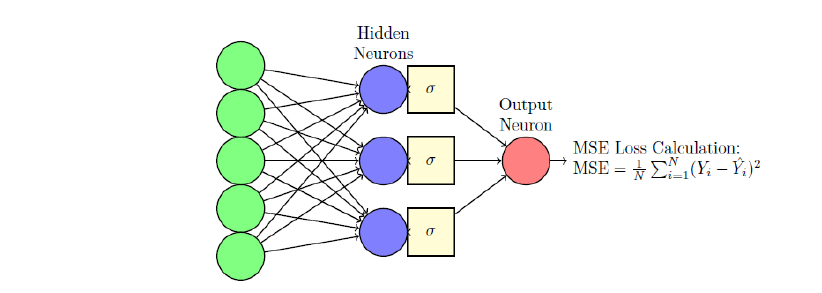
\includegraphics[scale=0.5]{nn1.png}
\end{center}
In a one-layer Multi-Layer Perceptron (MLP) with a single hidden layer, we represent the weights as matrices
to efficiently handle the numerous connections between layers. For a network with m input neurons and n
hidden neurons, the weights and biases are defined as follows:
\begin{itemize}
    \item Weights of the Hidden Layer ($\mathbf{W}_h$): An $m \times n$ matrix.
    \item Biases of the Hidden Layer ($\mathbf{b}_h$): An $n$-dimensional vector.
    \item Weights of the Output Layer ($\mathbf{W}_o$): An $n \times k$ matrix (assuming $k$ output neurons).
    \item Biases of the Output Layer ($\mathbf{b}_o$): A $k$-dimensional vector.
\end{itemize}

The sigmoid activation function is defined as:
\[
\sigma(x) = \frac{1}{1 + e^{-x}}
\]

Its derivative, which is used in the computation of the gradient, is:
\[
\sigma'(x) = \sigma(x)(1 - \sigma(x))
\]

The Mean Squared Error (MSE) loss function is:
\[
MSE = \frac{1}{N} \sum_{i=1}^{N} (Y_i - \hat{Y}_i)^2
\]

where N is the number of samples, Y is the true output, and \(\hat{Y}\) is the predicted output.
\\ forward pass
\[
\mathbf{h} = \sigma(\mathbf{X} \mathbf{W}_h + \mathbf{b}_h)
\]
\textbf{Write down the gradients of the MSE with respect to the following parameters (15 points):}
the gradient of the loss w.r.t to the predicted output $\hat{Y}$ is:
\[
\frac{\partial MSE}{\partial \hat{Y}} = \frac{1}{N} \sum_{i=1}^{N} \frac{\partial}{\partial \hat{Y}} (Y_i - \hat{Y}_i)^2
\]
\[
\frac{\partial MSE}{\partial \hat{Y}} = \frac{1}{N} \sum_{i=1}^{N} -2(Y_i - \hat{Y}_i) = -\frac{2}{N} \sum_{i=1}^{N} (\hat{Y}_i - Y_i)
\]
\begin{enumerate}
    \item Gradient with respect to $\mathbf{W}_o$: $$\frac{\partial MSE}{\partial \mathbf{W}_o}$$
    the forward equation here is:
    \[
    \hat{Y} = \mathbf{\hat{h}} \mathbf{W}_o + \mathbf{b}_o
    \]
    so the gradient of the loss w.r.t to the weight $\mathbf{W}_o$ is:
    \[
    \frac{\partial MSE}{\partial \mathbf{W}_o} = \frac{\partial MSE}{\partial \hat{Y}} \cdot \frac{\partial \hat{Y}}{\partial \mathbf{W}_o}
    \]
    \[
    \frac{\partial MSE}{\partial \mathbf{W}_o} = -\frac{2}{N} \sum_{i=1}^{N} (\hat{Y}_i - Y_i) \cdot \frac{\partial}{\partial \mathbf{W}_o} (\mathbf{\hat{h}}_i \mathbf{W}_o + \mathbf{b}_o)
    \]
    \[
    \frac{\partial MSE}{\partial \mathbf{W}_o} = \mathbf{-\frac{2}{N} \sum_{i=1}^{N} (\hat{Y}_i - Y_i) \cdot \mathbf{\hat{h}}_i}
    \]
    
    \item Gradient with respect to $\mathbf{b}_o$: $$\frac{\partial MSE}{\partial \mathbf{b}_o}$$
    \[
        \frac{\partial MSE}{\partial \mathbf{b}_o} = \frac{\partial MSE}{\partial \hat{Y}} \cdot \frac{\partial \hat{Y}}{\partial \mathbf{b}_o}
        \]
        \[
            \frac{\partial MSE}{\partial \mathbf{b}_o} = -\frac{2}{N} \sum_{i=1}^{N} (\hat{Y}_i - Y_i) \cdot \frac{\partial}{\partial \mathbf{b}_o} (\mathbf{\hat{h}}_i \mathbf{W}_o + \mathbf{b}_o)
            \]
            \[
                \frac{\partial MSE}{\partial \mathbf{b}_o} = -\frac{2}{N} \sum_{i=1}^{N} (\hat{Y}_i - Y_i) \cdot 1 = \mathbf{-\frac{2}{N} \sum_{i=1}^{N} (\hat{Y}_i - Y_i)}
                \]
    \item Gradient with respect to $\mathbf{W}_h$: $$\frac{\partial MSE}{\partial \mathbf{W}_h}$$
    the forward equation for the hidden layer is: $\mathbf{\hat{h}} = \sigma(h)$ where $h = \mathbf{X} \mathbf{W}_h + \mathbf{b}_h$ 
    \\ Gradient of the M.S.E loss with respect to the output of the hidden layer $\hat{h}$ is:
    \[
    \frac{\partial MSE}{\partial \mathbf{\hat{h}}} = \frac{\partial MSE}{\partial \hat{Y}} \cdot \frac{\partial \hat{Y}}{\partial \mathbf{\hat{h}}}
    \]
    \[
    \frac{\partial MSE}{\partial \mathbf{\hat{h}}} = \frac{\partial MSE}{\partial \hat{Y}} \cdot \frac{\partial \hat{Y}}{\partial \mathbf{\hat{h}}} = \frac{\partial MSE}{\partial \hat{Y}} \cdot \mathbf{W}_o
    \]
    derivative of the loss w.r.t to sigmoid:
    \[
    \frac{\partial MSE}{\partial \sigma} = \frac{\partial MSE}{\partial \mathbf{\hat{h}}} \cdot \frac{\partial \mathbf{\hat{h}}}{\partial \sigma}
    \]
    but the derivative of the sigmoid function is $\sigma'(x) = \sigma(x)(1 - \sigma(x))$, so :
    \[
        \frac{\partial \mathbf{\hat{h}}}{\partial \sigma} = \mathbf{\hat{h}} \cdot (1 - \mathbf{\hat{h}})
    \]
    so:
    \[
        \frac{\partial \mathbf{\hat{h}}}{\partial \sigma} = \frac{\partial MSE}{\partial \mathbf{\hat{h}}} \cdot \frac{\partial \mathbf{\hat{h}}}{\partial \sigma} = \frac{\partial MSE}{\partial \mathbf{\hat{h}}} \cdot \mathbf{\hat{h}} \cdot (1 - \mathbf{\hat{h}})
    \]
    finally, the gradient of the loss w.r.t to the weight $\mathbf{W}_h$ is:
    \[
    \frac{\partial MSE}{\partial \mathbf{W}_h} = \frac{\partial MSE}{\partial \sigma} \cdot \frac{\partial \sigma}{\partial \mathbf{W}_h}
    \]
    \[
    \frac{\partial \sigma}{\partial \mathbf{W}_h} = \frac{\partial \sigma}{\partial h} \cdot \frac{\partial h}{\partial \mathbf{W}_h}
    \]
    \[
    \frac{\partial \sigma}{\partial \mathbf{W_h}} = \mathbf{X}
    \]
    the final derivative is:
    \[
    \frac{\partial MSE}{\partial \mathbf{W}_h} = \frac{\partial MSE}{\partial \sigma} \cdot \frac{\partial \sigma}{\partial \mathbf{W}_h} = \frac{\partial MSE}{\partial \mathbf{\hat{h}}} \cdot \frac{\partial \mathbf{\hat{h}}}{\partial \sigma} \cdot \frac{\partial \sigma}{\partial \mathbf{W}_h}
    \]
    \[
    = \frac{\partial MSE}{\partial \mathbf{\hat{h}}} \cdot \mathbf{\hat{h}} \cdot (1 - \mathbf{\hat{h}}) \cdot \mathbf{X}
    \]
    where $\frac{\partial MSE}{\partial \mathbf{\hat{h}}}$ is defined above
    \item Gradient with respect to $\mathbf{b}_h$: $$\frac{\partial MSE}{\partial \mathbf{b}_h}$$
    \[
    \frac{\partial MSE}{\partial \mathbf{b}_h} = \frac{\partial MSE}{\partial \sigma} \cdot \frac{\partial \sigma}{\partial \mathbf{b}_h}
    \]
    \[
    \frac{\partial \sigma}{\partial \mathbf{b}_h} = 1 
    \]
    the final derivative is:
    \[
    \frac{\partial MSE}{\partial \mathbf{b}_h} = \frac{\partial MSE}{\partial \sigma} \cdot \frac{\partial \sigma}{\partial \mathbf{b}_h} = \frac{\partial MSE}{\partial \mathbf{\hat{h}}} \cdot \hat{h} \cdot (1 - \hat{h})
    \]
    where $\frac{\partial MSE}{\partial \mathbf{\hat{h}}}$ is defined above
\end{enumerate}

Write down the gradient descent update rules for the parameters using a learning rate of 0.1 (5 points).
\[
w_{\text{new}} = w_{\text{old}} - \alpha \cdot \nabla_w L,
\]
\[
b_{\text{new}} = b_{\text{old}} - \alpha \cdot \nabla_b L,
\]

\[
\text{where } w \text{ represents the weights and } b \text{ represents the biases.}
\]

For the $\mathbf{W}_h$ and $\mathbf{W}_o$ matrices, the update rules are:
\[
\mathbf{W}_{h_{\text{new}}} = \mathbf{W}_{h_{\text{old}}} - \alpha \cdot \nabla_{\mathbf{W}_h} L,
\]
\[
\mathbf{W}_{o_{\text{new}}} = \mathbf{W}_{o_{\text{old}}} - \alpha \cdot \nabla_{\mathbf{W}_o} L,
\]

for the $\mathbf{b}_h$ and $\mathbf{b}_o$ vectors, the update rules are:

\[
\mathbf{b}_{h_{\text{new}}} = \mathbf{b}_{h_{\text{old}}} - \alpha \cdot \nabla_{\mathbf{b}_h} L,
\]
\[
\mathbf{b}_{o_{\text{new}}} = \mathbf{b}_{o_{\text{old}}} - \alpha \cdot \nabla_{\mathbf{b}_o} L,
\]

Complete the MLP codes in the starter notebook (20 points).

\textbf{Bonus (10 points):} Add Another layer hidden layer to MLP. and complete the codes in the 2 Layer MLP.
You should still use sigmoid activation on the new layer. What is the effect of adding another layer ?

\section{Evaluations (10 Points)}
In class, we discussed solving a linear regression using the pseudo-inverse, which gives the same result as minimizing the residual sum of squares. In the starter notebook, I have provided a solution to the linear regression problem using SVD and the pseudo-inverse. Compare the root mean square error (RMSE) of this method, the ridge regression method, and the one-layer MLP. Why do you think the errors are different ?
Which one has the lowest error and why ?

I have provided a keras implementation of a deeper neural network with 4 layers and it ouputs the lowers
RMSE error. However, there are some techniques added here like dropout, weight initialization, different
activation function, and Adam optimizer (we used SGD optimizer in previous question). If you are interested
in knowing more about deep neural networks, then you should consider taking the course introduction to
deep learning offered here at CMU by Prof Bhiksha.
\end{document}